% Aberdeen style guide should be followed when using this
% layout. Their template powerpoint slide is used to extract the
% Aberdeen color and logo but is otherwise ignored (it has little or
% no formatting in it anyway).
%
% http://www.abdn.ac.uk/documents/style-guide.pdf

%%%%%%%%%%%%%%%%%%%% Document Class Settings %%%%%%%%%%%%%%%%%%%%%%%%%
% Pick if you want slides, or draft slides (no animations)
%%%%%%%%%%%%%%%%%%%%%%%%%%%%%%%%%%%%%%%%%%%%%%%%%%%%%%%%%%%%%%%%%%%%%%
%Normal document mode%
\documentclass[10pt,compress]{beamer}
%Draft or handout mode
%\documentclass[10pt,compress,handout]{beamer}
%\documentclass[10pt,compress,handout,ignorenonframetext]{beamer}

%%%%%%%%%%%%%%%%%%%% General Document settings %%%%%%%%%%%%%%%%%%%%%%%
% These settings must be set for each presentation
%%%%%%%%%%%%%%%%%%%%%%%%%%%%%%%%%%%%%%%%%%%%%%%%%%%%%%%%%%%%%%%%%%%%%%
\newcommand{\shortname}{jefferson.gomes@abdn.ac.uk}
\newcommand{\fullname}{Dr Jeff Gomes}
\institute{School of Engineering}
\newcommand{\emailaddress}{}%jefferson.gomes@abdn.ac.uk}
\newcommand{\logoimage}{../FigBanner/UoAHorizBanner}
\title{Heat, Mass and Momentum Transfer $\&$ Thermodynamics2 (EX3030/EM40JK)}
\subtitle{Design of Heat Exchangers}
%\subtitle{Module 1.1: Review of Thermodynamics}
\date[ ]{ }

%%%%%%%%%%%%%%%%%%%% Template settings %%%%%%%%%%%%%%%%%%%%%%%%%%%%%%%
% You shouldn't have to change below this line, unless you want to.
%%%%%%%%%%%%%%%%%%%%%%%%%%%%%%%%%%%%%%%%%%%%%%%%%%%%%%%%%%%%%%%%%%%%%%
\usecolortheme{whale}
\useoutertheme{infolines}

% Use the fading effect for items that are covered on the current
% slide.
\beamertemplatetransparentcovered

% We abuse the author command to place all of the slide information on
% the title page.
\author[\shortname]{%
  \fullname\\\ttfamily{\emailaddress}
}


%At the start of every section, put a slide indicating the contents of the current section.
\AtBeginSection[] {
  \begin{frame}
    \frametitle{Section Outline}
    \tableofcontents[currentsection]
  \end{frame}
}

% Allow the inclusion of movies into the Presentation! At present,
% only the Okular program is capable of playing the movies *IN* the
% presentation.
\usepackage{multimedia}
\usepackage{animate}

%% Handsout -- comment out the lines below to create handstout with 4 slides in a page with space for comments
\usepackage{handoutWithNotes}

\mode<handout>
{
\usepackage{pgf,pgfpages}

\pgfpagesdeclarelayout{2 on 1 boxed with notes}
{
\edef\pgfpageoptionheight{\the\paperheight} 
\edef\pgfpageoptionwidth{\the\paperwidth}
\edef\pgfpageoptionborder{0pt}
}
{
\setkeys{pgfpagesuselayoutoption}{landscape}
\pgfpagesphysicalpageoptions
    {%
        logical pages=4,%
        physical height=\pgfpageoptionheight,%
        physical width=\pgfpageoptionwidth,%
        last logical shipout=2%
    } 
\pgfpageslogicalpageoptions{1}
    {%
    border code=\pgfsetlinewidth{1pt}\pgfstroke,%
    scale=1,
    center=\pgfpoint{.25\pgfphysicalwidth}{.75\pgfphysicalheight}%
    }%
\pgfpageslogicalpageoptions{2}
    {%
    border code=\pgfsetlinewidth{1pt}\pgfstroke,%
    scale=1,
    center=\pgfpoint{.25\pgfphysicalwidth}{.25\pgfphysicalheight}%
    }%
\pgfpageslogicalpageoptions{3}
    {%
    border shrink=\pgfpageoptionborder,%
    resized width=.7\pgfphysicalwidth,%
    resized height=.5\pgfphysicalheight,%
    center=\pgfpoint{.75\pgfphysicalwidth}{.29\pgfphysicalheight},%
    copy from=3
    }%
\pgfpageslogicalpageoptions{4}
    {%
    border shrink=\pgfpageoptionborder,%
    resized width=.7\pgfphysicalwidth,%
    resized height=.5\pgfphysicalheight,%
    center=\pgfpoint{.75\pgfphysicalwidth}{.79\pgfphysicalheight},%
    copy from=4
    }%

\AtBeginDocument
    {
    \newbox\notesbox
    \setbox\notesbox=\vbox
        {
            \hsize=\paperwidth
            \vskip-1in\hskip-1in\vbox
            {
                \vskip1cm
                Notes\vskip1cm
                        \hrule width\paperwidth\vskip1cm
                    \hrule width\paperwidth\vskip1cm
                        \hrule width\paperwidth\vskip1cm
                    \hrule width\paperwidth\vskip1cm
                        \hrule width\paperwidth\vskip1cm
                    \hrule width\paperwidth\vskip1cm
                    \hrule width\paperwidth\vskip1cm
                    \hrule width\paperwidth\vskip1cm
                        \hrule width\paperwidth
            }
        }
        \pgfpagesshipoutlogicalpage{3}\copy\notesbox
        \pgfpagesshipoutlogicalpage{4}\copy\notesbox
    }
}
}

%\pgfpagesuselayout{2 on 1 boxed with notes}[letterpaper,border shrink=5mm]
%\pgfpagesuselayout{2 on 1 boxed with notes}[letterpaper,border shrink=5mm]



%%%%% Color settings
\usepackage{color}
%% The background color for code listings (i.e. example programs)
\definecolor{lbcolor}{rgb}{0.9,0.9,0.9}%
\definecolor{UoARed}{rgb}{0.64706, 0.0, 0.12941}
\definecolor{UoALight}{rgb}{0.85, 0.85, 0.85}
\definecolor{UoALighter}{rgb}{0.92, 0.92, 0.92}
\setbeamercolor{structure}{fg=UoARed} % General background and higlight color
\setbeamercolor{frametitle}{bg=black} % General color
\setbeamercolor{frametitle right}{bg=black} % General color
\setbeamercolor{block body}{bg=UoALighter} % For blocks
\setbeamercolor{structure}{bg=UoALight} % For blocks
% Rounded boxes for blocks
\setbeamertemplate{blocks}[rounded]

%%%%% Font settings
% Aberdeen requires the use of Arial in slides. We can use the
% Helvetica font as its widely available like so
% \usepackage{helvet}
% \renewcommand{\familydefault}{\sfdefault}
% But beamer already uses a sans font, so we will stick with that.

% The size of the font used for the code listings.
\newcommand{\goodsize}{\fontsize{6}{7}\selectfont}

% Extra math packages, symbols and colors. If you're using Latex you
% must be using it for formatting the math!
\usepackage{amscd,amssymb} \usepackage{amsfonts}
\usepackage[mathscr]{eucal} \usepackage{mathrsfs}
\usepackage{latexsym} \usepackage{amsmath} \usepackage{bm}
\usepackage{amsthm} \usepackage{textcomp} \usepackage{eurosym}
% This package provides \cancel{a} and \cancelto{a}{b} to "cancel"
% expressions in math.
\usepackage{cancel}

\usepackage{comment} 

% Get rid of font warnings as modern LaTaX installations have scalable
% fonts
\usepackage{type1cm} 

%\usepackage{enumitem} % continuous numbering throughout enumerate commands

% For exact placement of images/text on the cover page
\usepackage[absolute]{textpos}
\setlength{\TPHorizModule}{1mm}%sets the textpos unit
\setlength{\TPVertModule}{\TPHorizModule} 

% Source code formatting package
\usepackage{listings}%
\lstset{ backgroundcolor=\color{lbcolor}, tabsize=4,
  numberstyle=\tiny, rulecolor=, language=C++, basicstyle=\goodsize,
  upquote=true, aboveskip={1.5\baselineskip}, columns=fixed,
  showstringspaces=false, extendedchars=true, breaklines=false,
  prebreak = \raisebox{0ex}[0ex][0ex]{\ensuremath{\hookleftarrow}},
  frame=single, showtabs=false, showspaces=false,
  showstringspaces=false, identifierstyle=\ttfamily,
  keywordstyle=\color[rgb]{0,0,1},
  commentstyle=\color[rgb]{0.133,0.545,0.133},
  stringstyle=\color[rgb]{0.627,0.126,0.941}}

% Allows the inclusion of other PDF's into the final PDF. Great for
% attaching tutorial sheets etc.
\usepackage{pdfpages}
\setbeamercolor{background canvas}{bg=}  

% Remove foot note horizontal rules, they occupy too much space on the slide
\renewcommand{\footnoterule}{}

% Force the driver to fix the colors on PDF's which include mixed
% colorspaces and transparency.
\pdfpageattr {/Group << /S /Transparency /I true /CS /DeviceRGB>>}

% Include a graphics, reserve space for it but
% show it on the next frame.
% Parameters:
% #1 Which slide you want it on
% #2 Previous slides
% #3 Options to \includegraphics (optional)
% #4 Name of graphic
\newcommand{\reserveandshow}[4]{%
\phantom{\includegraphics<#2|handout:0>[#3]{#4}}%
\includegraphics<#1>[#3]{#4}%
}
\usepackage{xcolor}

\newlength{\overwritelength}
\newlength{\minimumoverwritelength}
\setlength{\minimumoverwritelength}{1cm}
\newcommand{\overwrite}[3][red]{%
  \settowidth{\overwritelength}{$#2$}%
  \ifdim\overwritelength<\minimumoverwritelength%
    \setlength{\overwritelength}{\minimumoverwritelength}\fi%
  \stackrel
    {%
      \begin{minipage}{\overwritelength}%
        \color{#1}\centering\small #3\\%
        \rule{1pt}{9pt}%
      \end{minipage}}
    {\colorbox{#1!50}{\color{black}$\displaystyle#2$}}} 

\newcommand{\frc}{\displaystyle\frac}
\newcommand{\red}{\textcolor{red}}
\newcommand{\blue}{\textcolor{blue}}
\newcommand{\green}{\textcolor{green}}
\newcommand{\purple}{\textcolor{purple}} 

\begin{document}

% Title page layout
\begin{frame}
  \titlepage
  \vfill%
  \begin{center}
    \includegraphics[clip,width=0.8\textwidth]{\logoimage}
  \end{center}
\end{frame}

% Table of contents
%\frame{ \frametitle{Slides Outline}
%  \tableofcontents
%}


%%%%%%%%%%%%%%%%%%%% The Presentation Proper %%%%%%%%%%%%%%%%%%%%%%%%%
% Fill below this line with \begin{frame} commands! It's best to
% always add the fragile option incase you're going to use the
% verbatim environment.
%%%%%%%%%%%%%%%%%%%%%%%%%%%%%%%%%%%%%%%%%%%%%%%%%%%%%%%%%%%%%%%%%%%%%%

%%%
%%% SECTION
%%%
\section{Introduction} 


%%% SUBSECTION
\subsection{Objectives}


%%%
%%% Slide
%%%
\begin{frame}
 \frametitle{Introduction}
    \begin{columns}
       \begin{column}[l]{0.58\linewidth}
         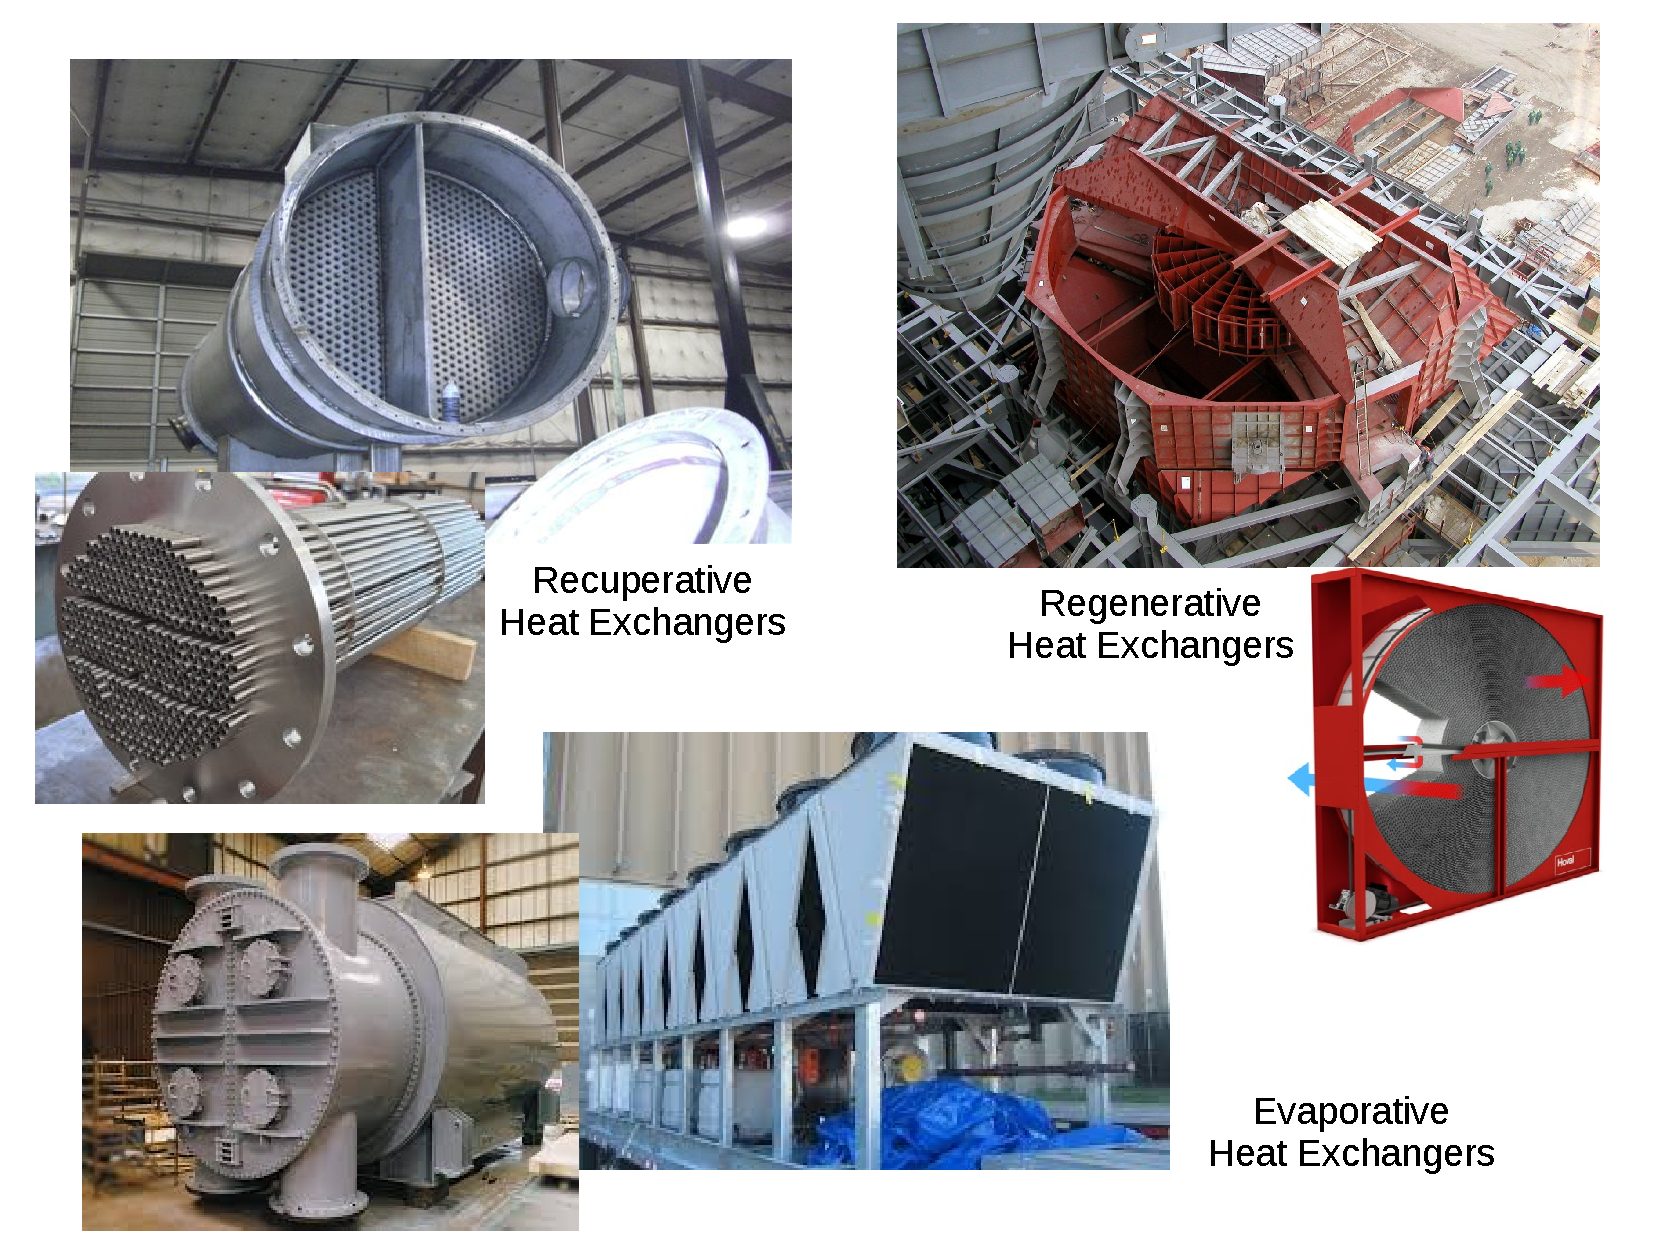
\includegraphics[width=1.1\columnwidth,clip]{./Pics/HeatExchangers_Examples}
       \end{column}
       \begin{column}[l]{0.42\linewidth}
          \begin{enumerate}\scriptsize
              \item<1-> Heat exchangers are devices used to transfer heat between two or more fluid streams at different temperatures;
              \item<2-> They are widely used in a number of industrial applications such as power generation, chemical processing, electronics cooling, refrigeration, and automotive;
              \item<3-> Heat exchangers (HE) are classified according to flow arrangement and type of construction.
              \item<3-> In general there are 3 main types of HE:
                \begin{enumerate}\scriptsize
                  \item<3-> \blue{Recuperative}: heat is transferred from one fluid to another through a dividing wall;
                  \item<3-> \blue{Regenerative}: heat from a hot fluid is stored in a thermal storage medium before being transferred to a cold fluid;
                  \item<3-> \blue{Evaporative}: heat from hot fluid is removed by partial evaporation.
                \end{enumerate}
               \item<4-> Our main focus on this module is to study \blue{Recuperative HE}.
          \end{enumerate}
       \end{column}      
    \end{columns}
\end{frame}

%%%
%%% SUBSECTION
%%%
\subsection{Bibliography} 

%%%
%%% Slide
%%%
\begin{frame}
 \frametitle{Suggested References}
  Literature relevant for this module:
  \begin{enumerate}[{[}1{]}]
    \item F.P. Incropera, D.P. DeWitt, T.L.Bergman, A.S. Lavine, `Introduction to Heat Transfer' (John Willey $\&$ Sons): Chapter 11.
    \item J.P. Holman, `Heat Transfer', 10$^{th}$ Edition (McGraw-Hill): Chapter 10;
    \item Y.A. Cengel, `Heat Transfer: A Practical Approach', 2$^{nd}$ Edition (McGraw-Hill): Chapter 13;
    \item L. Theodore, `Essential Engineering Calculations Series: Heat Transfer Applications for the Practicing Engineer' (John Willey $\&$ Sons): Chapter 14.
  \end{enumerate}
\end{frame}

%%%
%%%  SECTION
%%%
\section{Design of Heat Exchangers}

%%% SUBSECTION
\subsection{Introduction}

%%%
%%% Slide
%%%
\begin{frame}
  \frametitle{Introduction}
    \begin{columns}
       \begin{column}[l]{0.5\linewidth}
         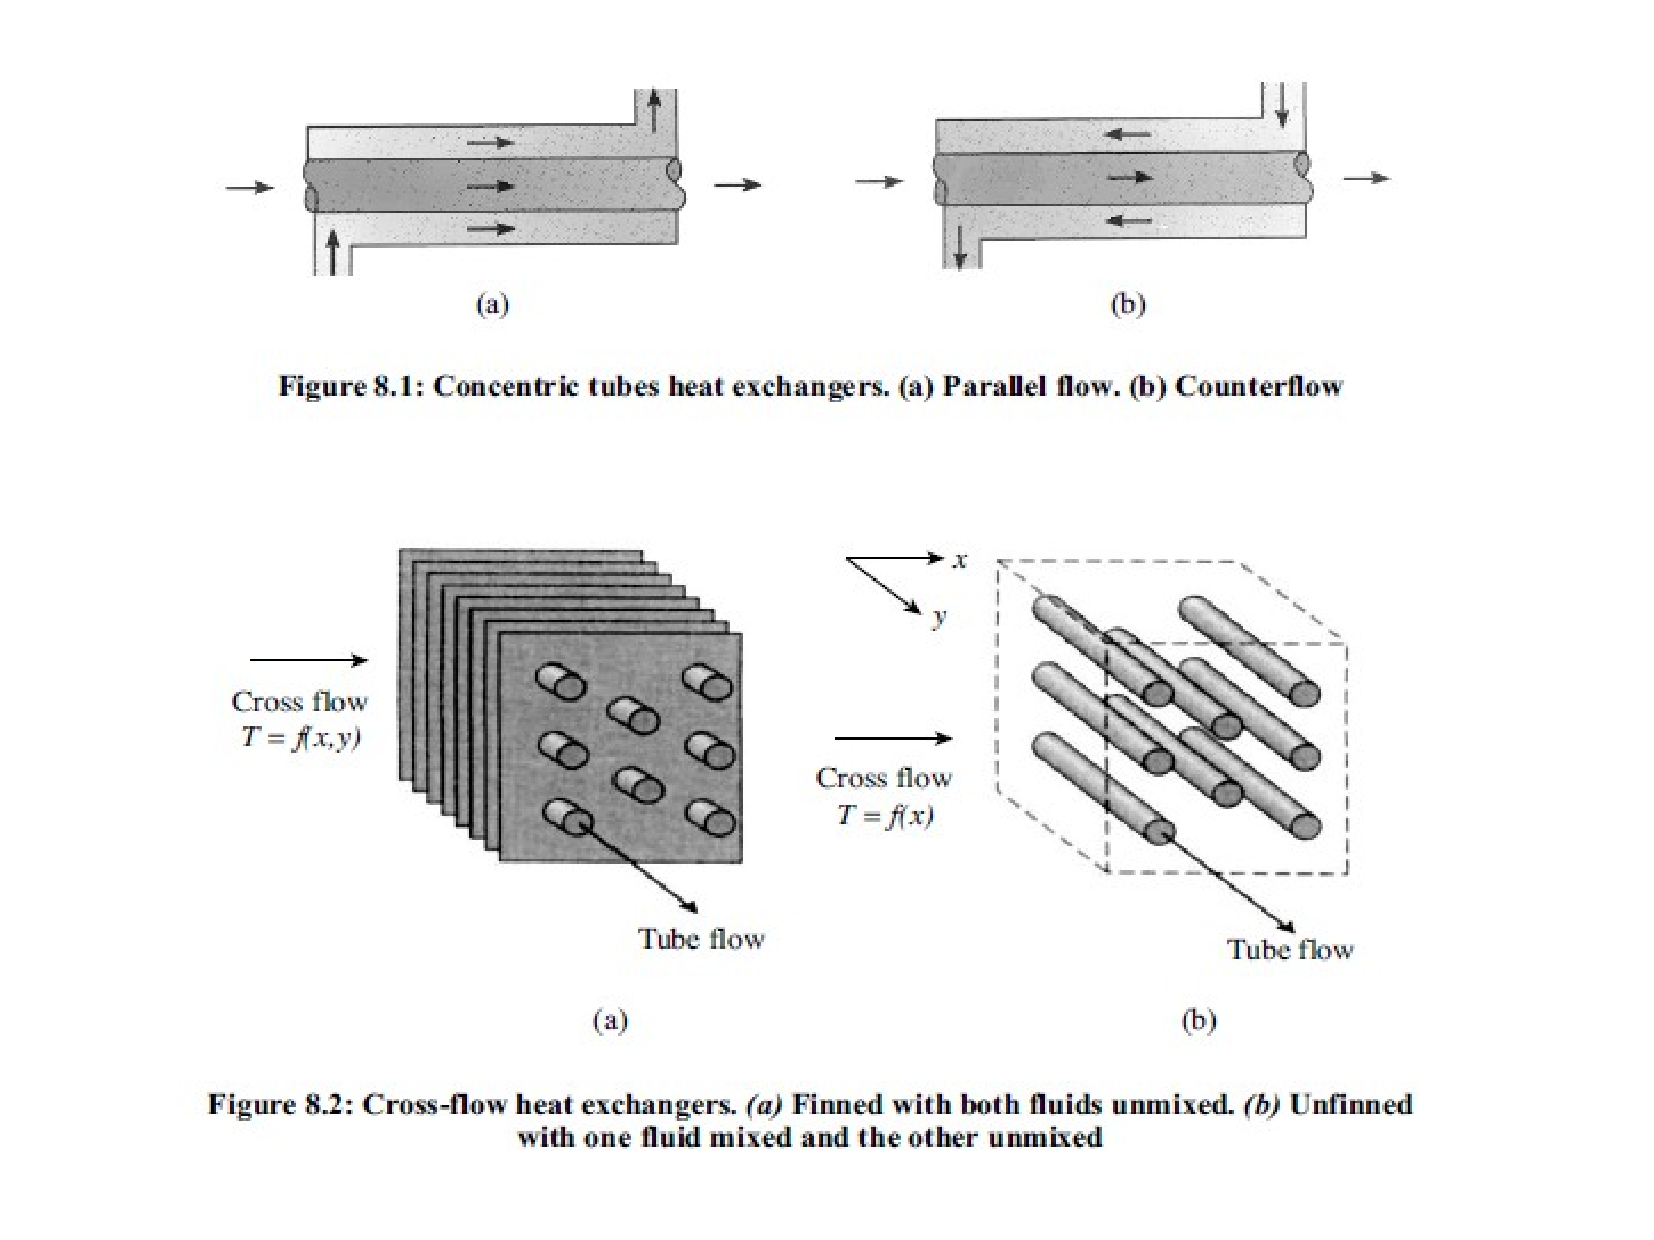
\includegraphics[width=1.3\columnwidth,clip]{./Pics/HeatExchangers_Classification}
       \end{column}
       \begin{column}[l]{0.5\linewidth}
         \begin{enumerate}\scriptsize
            \item<1-> The main objective of HE is to transfer heat from a fluid to another fluid;
            \item<1-> The basic configuration of a HE is a fluid flowing through a tube whereas another fluid (at different temperature) flows outside;
            \item<2-> Heat through this HE configuration occur via 3 mechanisms:
              \begin{enumerate}\scriptsize
                 \item<2-> Convective heat transfer from the fluid to the inner wall of the tube;
                 \item<2-> Conductive heat transfer through the tube wall and;
                 \item<2-> Convective heat transfer from the outer tube wall to the outside fluid.
              \end{enumerate}
            \item<3-> HE are typically classified according to flow arrangements and type of construction:
              \begin{enumerate}\scriptsize
                  \item<3-> Concentric tube (or double-pipe):
                       \begin{enumerate}\scriptsize
                          \item<3-> Parallel flow;
                          \item<3-> Counterflow;
                       \end{enumerate}
                  \item<3-> Cross-flow
              \end{enumerate}
         \end{enumerate}
       \end{column}      
    \end{columns}
\end{frame}


%%%
%%% Slide
%%%
\begin{frame}
  \frametitle{Introduction}
    \begin{center}
         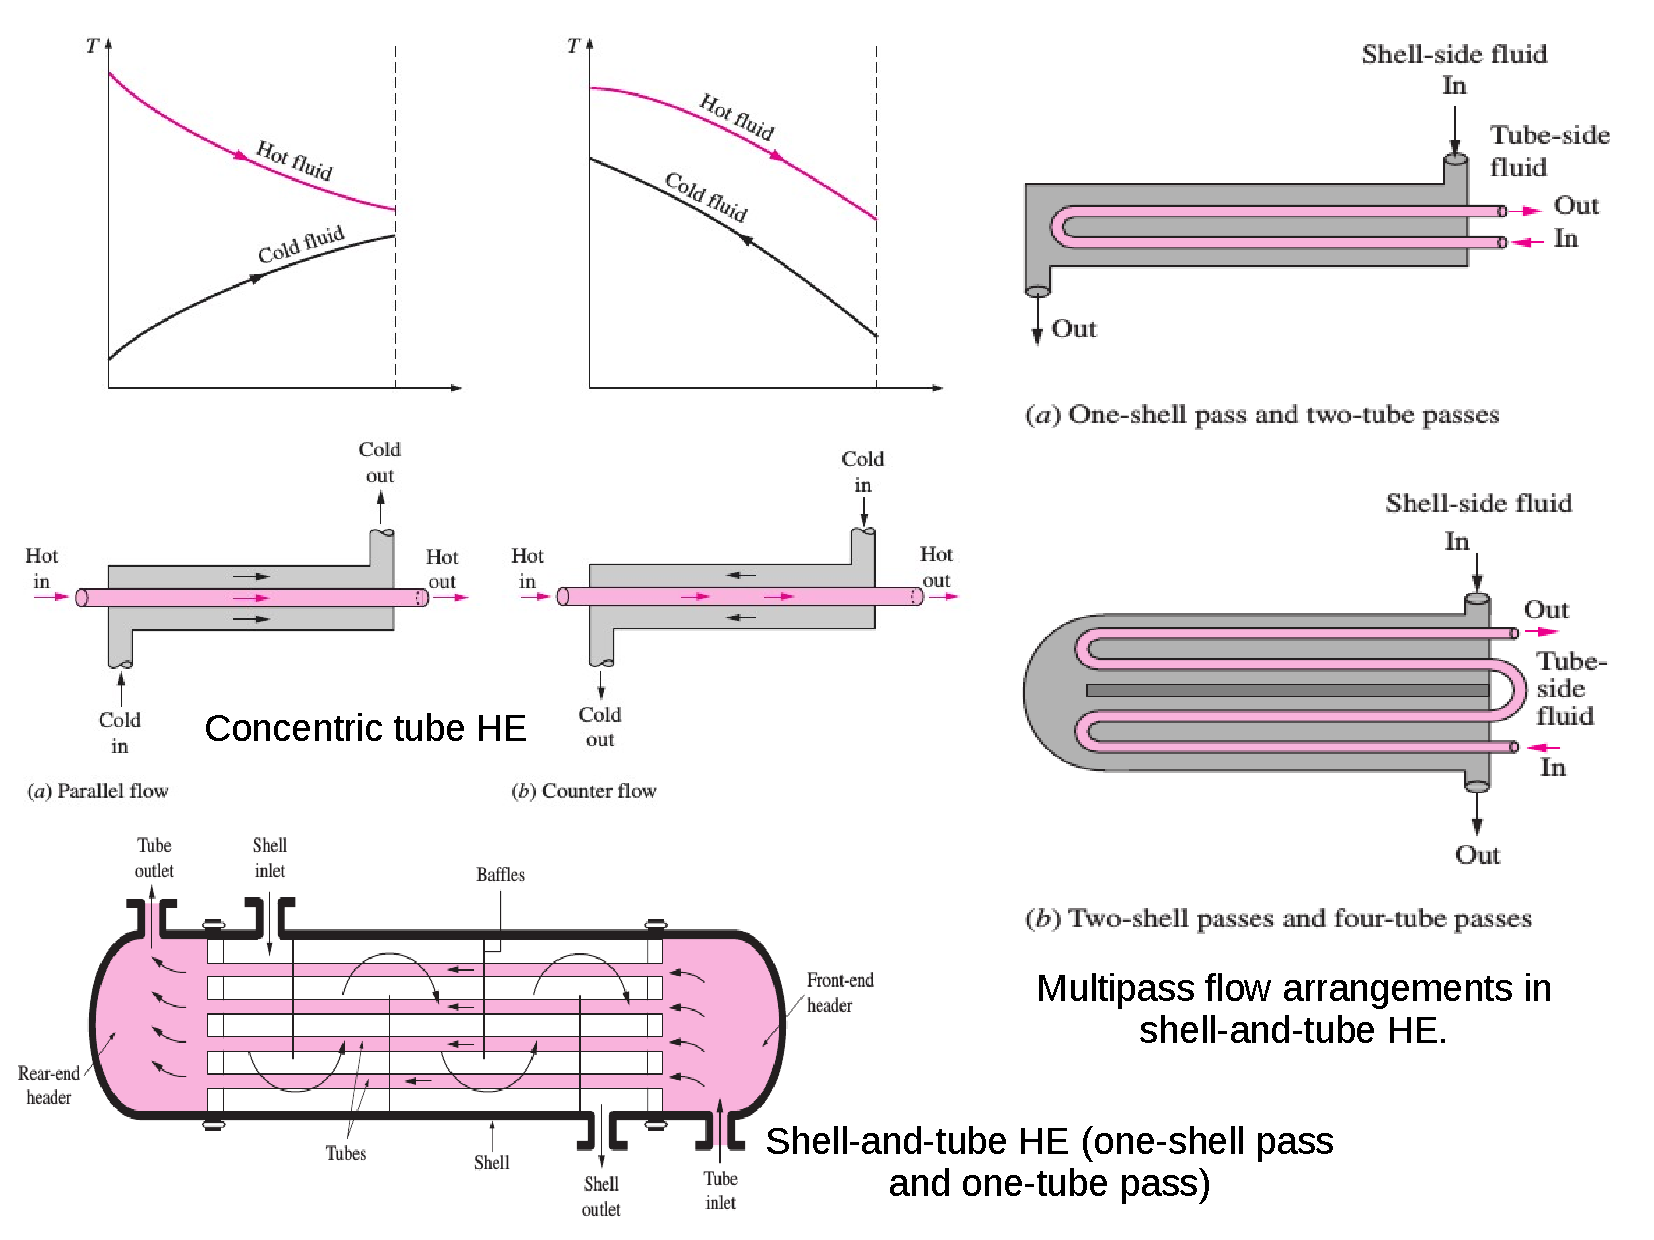
\includegraphics[width=1.\columnwidth,height=0.65\columnwidth,clip]{./Pics/HeatExchangers_Classification2}
    \end{center}
\end{frame}


%%% SUBSECTION
\subsection{Overall Heat Transfer Coefficient Calculations}

%%%
%%% Slide
%%%
\begin{frame}
  \frametitle{Overall Heat Transfer Coefficient Calculations}
    \begin{columns}
       \begin{column}[l]{0.5\linewidth}
         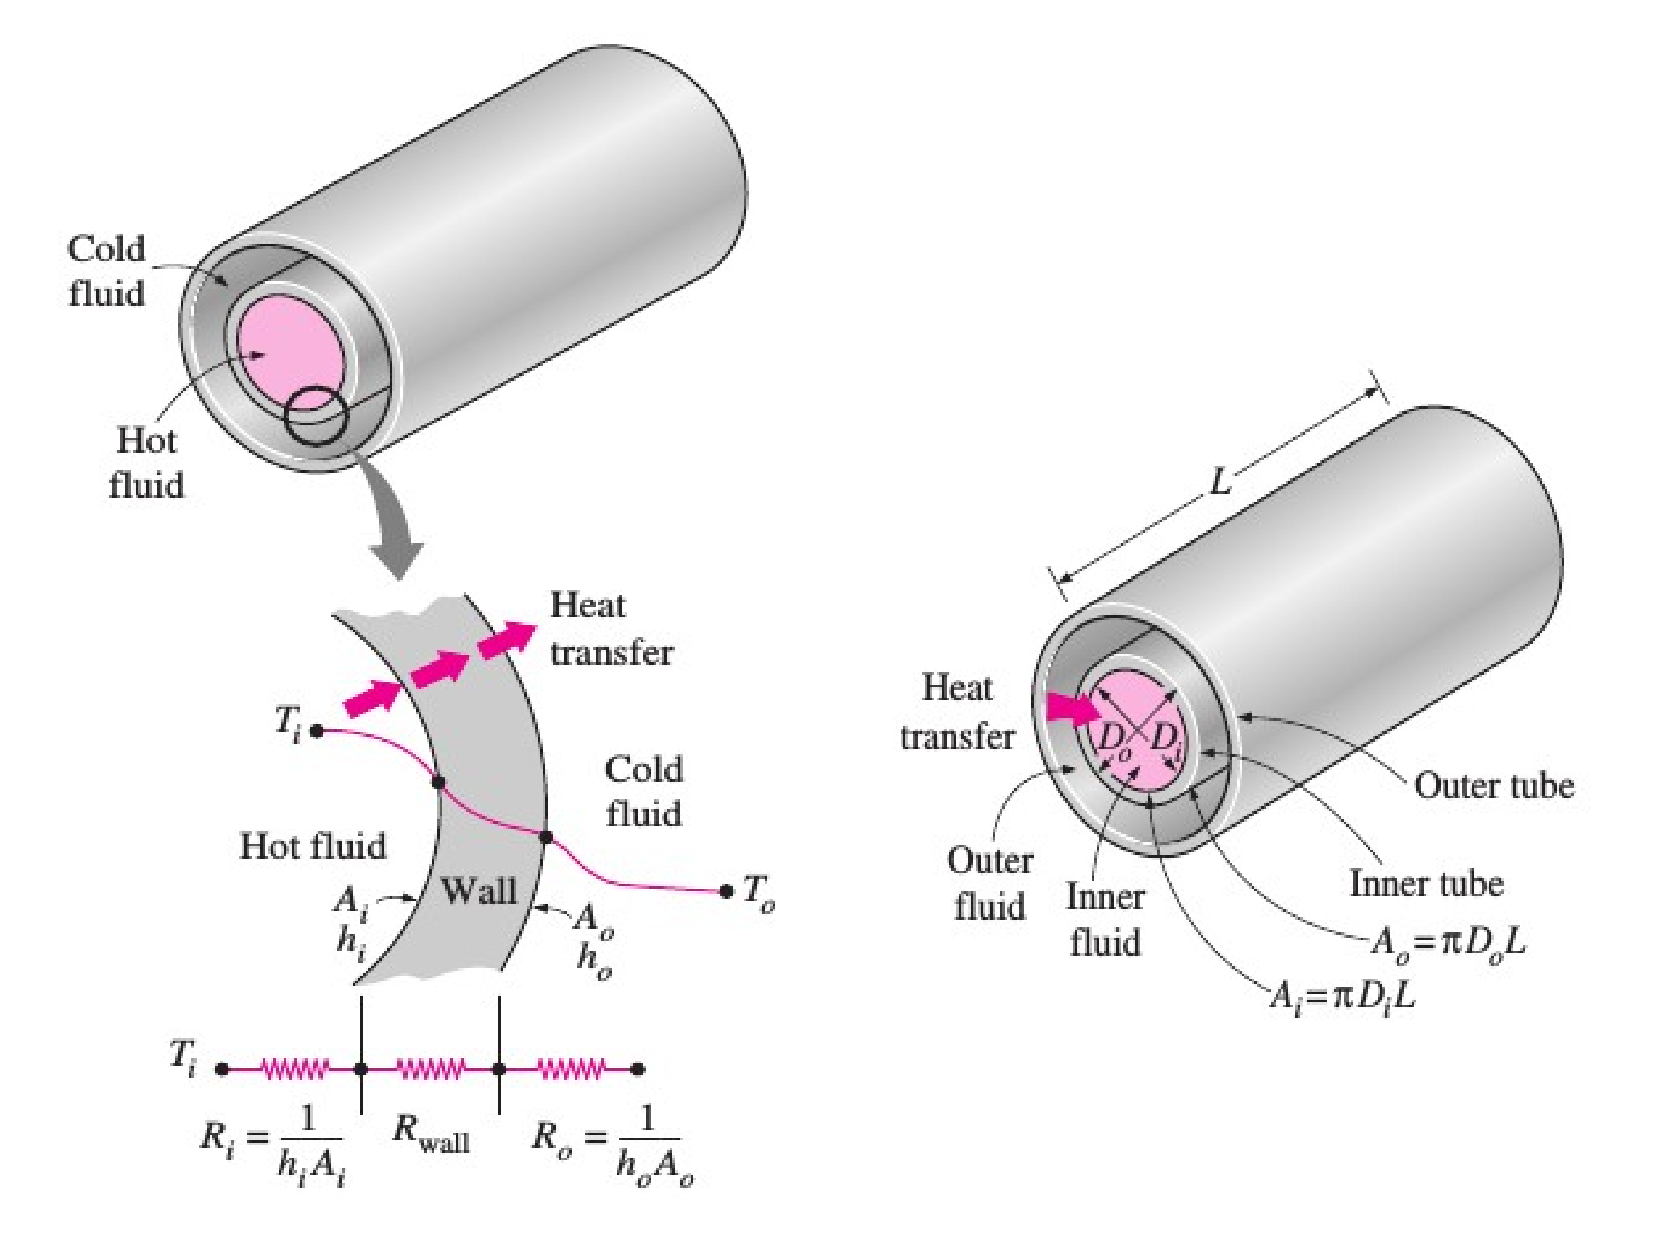
\includegraphics[width=1.1\columnwidth,clip]{./Pics/HeatExchangers_Flow}
         \begin{enumerate}\scriptsize
            \item<1-> In concentric tube HE, the heat exchange rate is
               \visible<1->{\begin{displaymath}
                  \dot{\mathcal{Q}} = \dot{m}_{c}C_{p,c}\left(T_{c,\text{out}}-T_{c,\text{in}}\right) = \dot{m}_{h}C_{p,h}\left(T_{h,\text{in}}-T_{h,\text{out}}\right) 
               \end{displaymath}
               where $\dot{m}$ is the mass flow rate.}
         \end{enumerate}
       \end{column}
       \begin{column}[l]{0.5\linewidth}
         \begin{enumerate}\setcounter{enumi}{1}\scriptsize
            %\item<2-> In \blue{condensers} and \blue{boilers}, fluids undertake a phase change with heat transfer rate of
            %   \visible<2->{\begin{displaymath}
            %     \dot{\mathcal{Q}} = \dot{m}h_{fg}
            %   \end{displaymath}   
            %   where $\dot{m}$ and $h_{fg}$ are the rate of vaporisation (or condensation) and the specific enthalpy of vaporisation.
            \item<2-> Assuming internal and outer superficial areas of $A_{i}=\pi D_{i}L$ and $A_{o}=\pi D_{o}L$, respectively, the \blue{thermal resistance} of the tube wall of length $L$ is
               \visible<2->{\begin{equation}
                  R_{\text{wall}} = \frc{\ln{D_{o}/D_{i}}}{2\pi \kappa L}
               \end{equation}}   
            \item<3-> The \blue{total thermal resistance}, \blue{$\mathcal{R}$} from the outer to the inner fluids is,
               \visible<3->{\begin{equation}
                  \mathcal{R} = R_{i} + R_{\text{wall}} + R_{o} = \frc{1}{h_{i}A_{i}} + \frc{\ln{D_{o}/D_{i}}}{2\pi \kappa L} + \frc{1}{h_{o}A_{o}} 
               \end{equation}}     
            \item<4-> Thus the heat transfer rate between the hot to the cold fluids can be expressed as,
               \visible<4->{\begin{equation}\label{HE:NewtonEqn}
                  \blue{\dot{\mathcal{Q}} =} \frc{\Delta T}{\mathcal{R}} = \blue{U A \Delta T} = U_{i}A_{i}\Delta T = U_{o}A_{o}\Delta T
               \end{equation}
               where \blue{$U$} is the \blue{overall heat transfer coefficient $\left(\text{W.m}^{-2}.^{\circ}\text{C}^{-1}\right)$}.}     

         \end{enumerate}
       \end{column}      
    \end{columns}
\end{frame}


%%%
%%% Slide
%%%
\begin{frame}
  \frametitle{Overall Heat Transfer Coefficient Calculations}
     \begin{enumerate}\setcounter{enumi}{4}\scriptsize
        \item<1-> Eliminating $\Delta T$ and inverting $\dot{\mathcal{Q}}$,
          \visible<1->{\begin{equation}
             \frc{1}{U_{i}A_{i}} = \frc{1}{U_{o}A_{o}} = \mathcal{R} \left(=\frc{1}{U A_{s}}\right) = \frc{1}{h_{i}A_{i}} + R_{\text{wall}} + \frc{1}{h_{o}A_{o}} \label{HE:Ucalc1}
          \end{equation}}
        \item<2-> If the wall thickness is small (in comparison with the length of the HE) with a large thermal conductivity, then the \blue{thermal wall resistance} is negligible $\left(\text{i.e., }R_{\text{wall}} \approx 0\right)$;
        \item<3-> Also, if $A_{i}\approx A_{o} \approx A_{s}$ (i.e., inner and outer diameters are very similar -- \blue{thin wall}),
          \visible<1->{\begin{equation}
             \frc{1}{U} \approx  \frc{1}{h_{i}} +  \frc{1}{h_{o}} \label{HE:Ucalc2}
          \end{equation}} 
     \end{enumerate}

     \visible<4->{\begin{block}{\begin{center}\scriptsize Fouling Factor\end{center}}\scriptsize
          \begin{equation}\scriptsize
             \frc{1}{U_{i}A_{i}} = \frc{1}{U_{o}A_{o}} = \mathcal{R} \left(=\frc{1}{U A_{s}}\right) = \frc{1}{h_{i}A_{i}} + \blue{\frc{R_{\text{f,i}}}{A_{i}}} + R_{\text{wall}} + \blue{\frc{R_{\text{f,o}}}{A_{o}}} + \frc{1}{h_{o}A_{o}} \label{HE:Ucalc3}
          \end{equation}
     \end{block}}

\end{frame}


%%%
%%% Slide (Cengel Example 13.1)
%%%
\begin{frame}
  \frametitle{Overall Heat Transfer Coefficient Calculations -- Example 1}
     \begin{enumerate}
          \item Hot oil is to be cooled in a double-tube counter-flow HE. The copper inner tubes have diameter of 2cm and negligible thickness. The inner diameter of the outer tube (shell) is 3cm. Water flows through the tube at a rate of 0.5 kg/s, and the oil through the shell at a rate of 0.8 kg/s. Taking the average temperatures of the water and the oil to be 45$^{\circ}$C and 80$^{\circ}$C, respectively, determine the overall heat transfer coefficient of this HE. Given, 
       \begin{enumerate}[(a)]
          \item Water at 45$^{\circ}$C: $\rho=990$kg/m$^{3}$, $\kappa=0.637$W/(m.K), $Pr=3.91$, $\nu=\mu/\rho=0.602\times 10^{-6}$m$^{2}$/s; 
          \item Oil at 80$^{\circ}$C: $\rho=852$kg/m$^{3}$, $\kappa=0.138$W/(m.K), $Pr=490$, $\nu=37.5\times 10^{-6}$m$^{2}$/s
       \end{enumerate}
     \end{enumerate}

\end{frame}


%%%
%%% Slide (Cengel Example 13.2)
%%%
\begin{frame}
  \frametitle{Overall Heat Transfer Coefficient Calculations -- Example 2}
     \begin{enumerate}\setcounter{enumi}{1}
          \item A double-pipe (shell-and-tube) heat exchanger is constructed of a stainless steel ($\kappa=$ 15.1 W/(m.$^{\circ}$C) inner tube of inner diameter D$_{i}=$ 1.5 cm and outer diameter D$_{o}=$ 1.9 cm and an outer shell of inner diameter 3.2 cm. The convective heat transfer coefficient is h$_{i}=$ 800 W/(m$^{2}.^{\circ}$C) on the inner surface of the tube and h$_{o}=$ 1200 W/(m$^{2}.^{\circ}$C) on the outer surface. For a fouling factor R$_{f,i}=$ 0.0004 m$^{2}.^{\circ}$C/W on the tube side and R$_{f,o}=$ 0.0001 m$^{2}.^{\circ}$C/W on the shell side, determine:
              \begin{enumerate}
                  \item The thermal resistance of the heat exchanger per unit length and; 
                  \item The overall heat transfer coefficients, U$_{i}$ and U$_{o}$ based on the inner and outer surface areas of the tube, respectively.
              \end{enumerate}

     \end{enumerate}

\end{frame}

%%%
%%% SUBSECTION
%%%

\subsection{Analysis Heat Exchangers}

%%%
%%% Slide 
%%%
\begin{frame}
  \frametitle{Introduction}
     \begin{enumerate}%\setcounter{enumi}{1}
          \item<1-> From energy conservation, the heat transfer rate in HE for the two fluid streams can be defined as
             \visible<1->{\begin{eqnarray}
               &&\dot{\mathcal{Q}}_{\text{hot}} + \dot{\mathcal{Q}}_{\text{cold}} = 0 \nonumber \\
               && \dot{m}_{\text{hot}}C_{p,\text{hot}}\left(T_{\text{hot,out}}-T_{\text{hot,in}}\right) + \dot{m}_{\text{cold}}C_{p,\text{cold}}\left(T_{\text{cold,out}}-T_{\text{cold,in}}\right) = 0 \label{HE:energyconservation}
             \end{eqnarray}}
          \item<2-> The product $\dot{m}_{i}C_{p,i}$ is called as {\it heat capacity rate} and represents the rate of heat transfer needed to change the temperature of the fluid by 1$^{\circ}$C as it flows through the HE;
          %\item<2-> Thus fluids with large {\it heat capacity rate} will produce {\it small temperature change};
          \item<2-> In the heat transfer rate equation in Eqn.~\ref{HE:NewtonEqn},
            \visible<2->{\begin{displaymath}
                \dot{Q} = U A \Delta T_{m}
            \end{displaymath}
            $\Delta T_{m}$ is an \blue{averaged} temperaterature difference between two fluids.}
          \item<3-> However $\Delta T_{m}$ and $U$ are not constants and vary along the HE. We can average $U$ by using the relations Eqns.~\ref{HE:Ucalc1}-\ref{HE:Ucalc3} and an average convective heat transfer coefficient for each fluid;
          \item<4-> For $\Delta T_{m}$, two methods are comonly used in thermal engineering systems:
             \begin{enumerate}
                \item<4-> Log-mean temperature difference method (or \blue{LMTD});
                \item<4-> Effectiveness-NTU method.
             \end{enumerate}
     \end{enumerate}

\end{frame}


%%%
%%% Slide 
%%%
\begin{frame}
  \frametitle{Log-mean Temperature Difference (LMTD) Method}
     \begin{enumerate}%\setcounter{enumi}{1}
          \item<1-> The energy conservation, Eqn.~\ref{HE:energyconservation} in differential form,
             \visible<1->{\begin{displaymath}
               d\dot{\mathcal{Q}}_{\text{hot}} + d\dot{\mathcal{Q}}_{\text{cold}} = 0 \Longrightarrow \dot{m}_{\text{cold}}C_{p,\text{cold}}dT_{\text{cold}} =  -\dot{m}_{\text{hot}}C_{p,\text{hot}}dT_{\text{hot}}.
             \end{displaymath}}
          \item<2-> After rearranging this equation and applying it into Eqn.~\ref{HE:NewtonEqn},
             \visible<2->{\begin{block}{\begin{center} LMTD Method\end{center}}
               \begin{equation}
                   \dot{\mathcal{Q}} = U A_{s} \Delta T_{\text{lm}}\;\text{ with }\;  \Delta T_{\text{lm}} = \frc{\left(T_{\text{hot,out}} - T_{\text{cold,out}}\right)-\left(T_{\text{hot,in}} - T_{\text{cold,in}}\right)}{\ln{\left(\frc{T_{\text{hot,out}} - T_{\text{cold,out}}}{T_{\text{hot,in}} - T_{\text{cold,in}}}\right)}}.
               \end{equation}
             \end{block} }
          \item<2-> For \blue{cross-flow and multipass shell-and-tube HE}, we need to use a correction factor, 
               \visible<2->{\begin{equation}
                   \dot{\mathcal{Q}} = U A_{s} F \Delta T_{\text{lm}},
               \end{equation}
               where the \blue{correction factor F} for different geometries can be found in {\it Appendix 1}.}
     \end{enumerate}

\end{frame}

%%%
%%% Slide 
%%%
\begin{frame}
  \frametitle{Log-mean Temperature Difference (LMTD) Method -- Example 3}
     \begin{enumerate}\setcounter{enumi}{2}
         \item Water at the rate of 68 kg/min is heated from 35 to 75$^{\circ}$C by an oil having a specific heat of 1.9 kJ/(kg.$^{\circ}$C). The fluids are used in a counterflow double-pipe HE, and the oil enters the exchanger at 110$^{\circ}$C and leaves at 75$^{\circ}$C. The overall heat-transfer coefficient is 320 W/(m$^{2}.^{\circ}$C). Given heat capacity of water (at constant pressure) of 4.18 kJ/(kg.$^{\circ}$C),
            \begin{enumerate}
               \item Calculate the HE area;
               \item Now assume that the HE is a shell-and-tube with water making one shell pass and the oil making two tube passes. Calculate the new HE. Assume that the overall heat-transfer coefficient remains the same.
            \end{enumerate}
     \end{enumerate}
\end{frame}

%%%
%%% Slide 
%%%
\begin{frame}
  \frametitle{The Effectiveness-NTU Method}
     \begin{enumerate}%\setcounter{enumi}{3}
          \item<1-> Given $T_{\text{i,j}}$, $\dot{m}_{i}$ (where $i = \left\{\text{hot,cold}\right\}$ and $j = \left\{\text{in,out}\right\}$) and $U$, we can readily determine the size (i.e., $A_{s}$) of the HE;
          \item<1-> The simplified algorithm is,
             \begin{enumerate}
                 \item<2-> Select the type of HE suitable for the process;
                 \item<2-> Determine any unknown inlet or outlet temperature and $\dot{\mathcal{Q}}$ through energy balance;
                 \item<2-> Calculate $\Delta T_{\text{lm}}$ (and $F$, if necessary);
                 \item<2-> Obtain \red{$U$};
                 \item<2-> Calculate \blue{$A_{s}$}. 
             \end{enumerate}
             \visible<3->{The selected HE has heat transfer surface area \blue{equal or larger than the calculated $A_{s}$}.}
          \item<4-> However, in most process designs we specify \blue{type} and \blue{size} of the HE, and determine some of the temperatures and mass flow rates for a prescribed \blue{heat transfer performance} of the HE;
          \item<5-> This would require intensive iterative methods;
     \end{enumerate}

\end{frame}


%%%
%%% Slide 
%%%
\begin{frame}
  \frametitle{The Effectiveness-NTU Method}
     \begin{enumerate}\setcounter{enumi}{4}
          \item<1-> The \blue{effectiveness-NTU method} was designed to simplify such HE analysis;
          \item<2-> The \blue{heat transfer effectiveness, $\epsilon$} is defined as
              \visible<2->{\begin{equation}
                \epsilon = \frc{\dot{\mathcal{Q}}}{\dot{\mathcal{Q}}_{\text{max}}} = \frc{\text{Actual heat transfer rate}}{\text{Maximum possible heat transfer rate}}
              \end{equation}}
          \item<2-> The {\it actual heat transfer rate} can be determined through energy balance;
          \item<3-> The {\it maximum possible heat transfer rate} is
              \visible<3->{\begin{equation}
                \dot{\mathcal{Q}}_{\text{max}} = \mathcal{C}_{\text{min}}\left(T_{\text{hot,in}}-T_{\text{cold,in}}\right)
              \end{equation}
              where $\mathcal{C}_{\text{min}} = Min\left\{\dot{m}_{\text{hot}}C_{p,\text{hot}}, \dot{m}_{\text{cold}}C_{p,\text{cold}}\right\}$}
          \item<4-> Effectiveness relations of HE often involve the dimensionless group $UA_{s}/C_{\text{min}}$, called \blue{number of transfer units (NTU)},
              \visible<4->{\begin{equation}
                \text{NTU} = \frc{UA_{s}}{C_{\text{min}}} = \frc{UA_{s}}{\left(\dot{m}C_{p}\right)_{\text{min}}}
              \end{equation}}         
     \end{enumerate}

\end{frame}

%%%
%%% Slide 
%%%
\begin{frame}
  \frametitle{The Effectiveness-NTU Method}
     \begin{enumerate}\setcounter{enumi}{9}
          \item<1-> Another important dimensionless quantity is the capacity ratio,
              \visible<1->{\begin{displaymath}
                 c = \frc{\mathcal{C}_{\text{min}}}{\mathcal{C}_{\text{max}}}
              \end{displaymath}}
          \item<2-> Therefore \blue{heat transfer effectiveness, $\epsilon$} can be expressed as a function of
              \visible<2->{\begin{displaymath}
                 \epsilon = \epsilon\left(UA_{s}/\mathcal{C}_{\text{min}}, \mathcal{C}_{\text{min}}/\mathcal{C}_{\text{max}}\right) = \epsilon\left(\text{NTU}, c\right)
              \end{displaymath}}
         
     \end{enumerate}

\end{frame}

%%%
%%% Slide 
%%%
\begin{frame}
  \frametitle{ The Effectiveness-NTU Method -- Example 4}
      \begin{enumerate}\setcounter{enumi}{3}
         \item For the HE of Example 3 with the same entering-fluid temperatures, calculate the exit water temperature when only 40 kg/min of water is heated but the same quantity of oil is used. Also calculate the total heat transfer under these new conditions.
      \end{enumerate}
\end{frame}

%%%
%%% Slide 
%%%
\begin{frame}
  \frametitle{ The Effectiveness-NTU Method -- Example 5}
    \begin{columns}
       \begin{column}[l]{0.58\linewidth}
         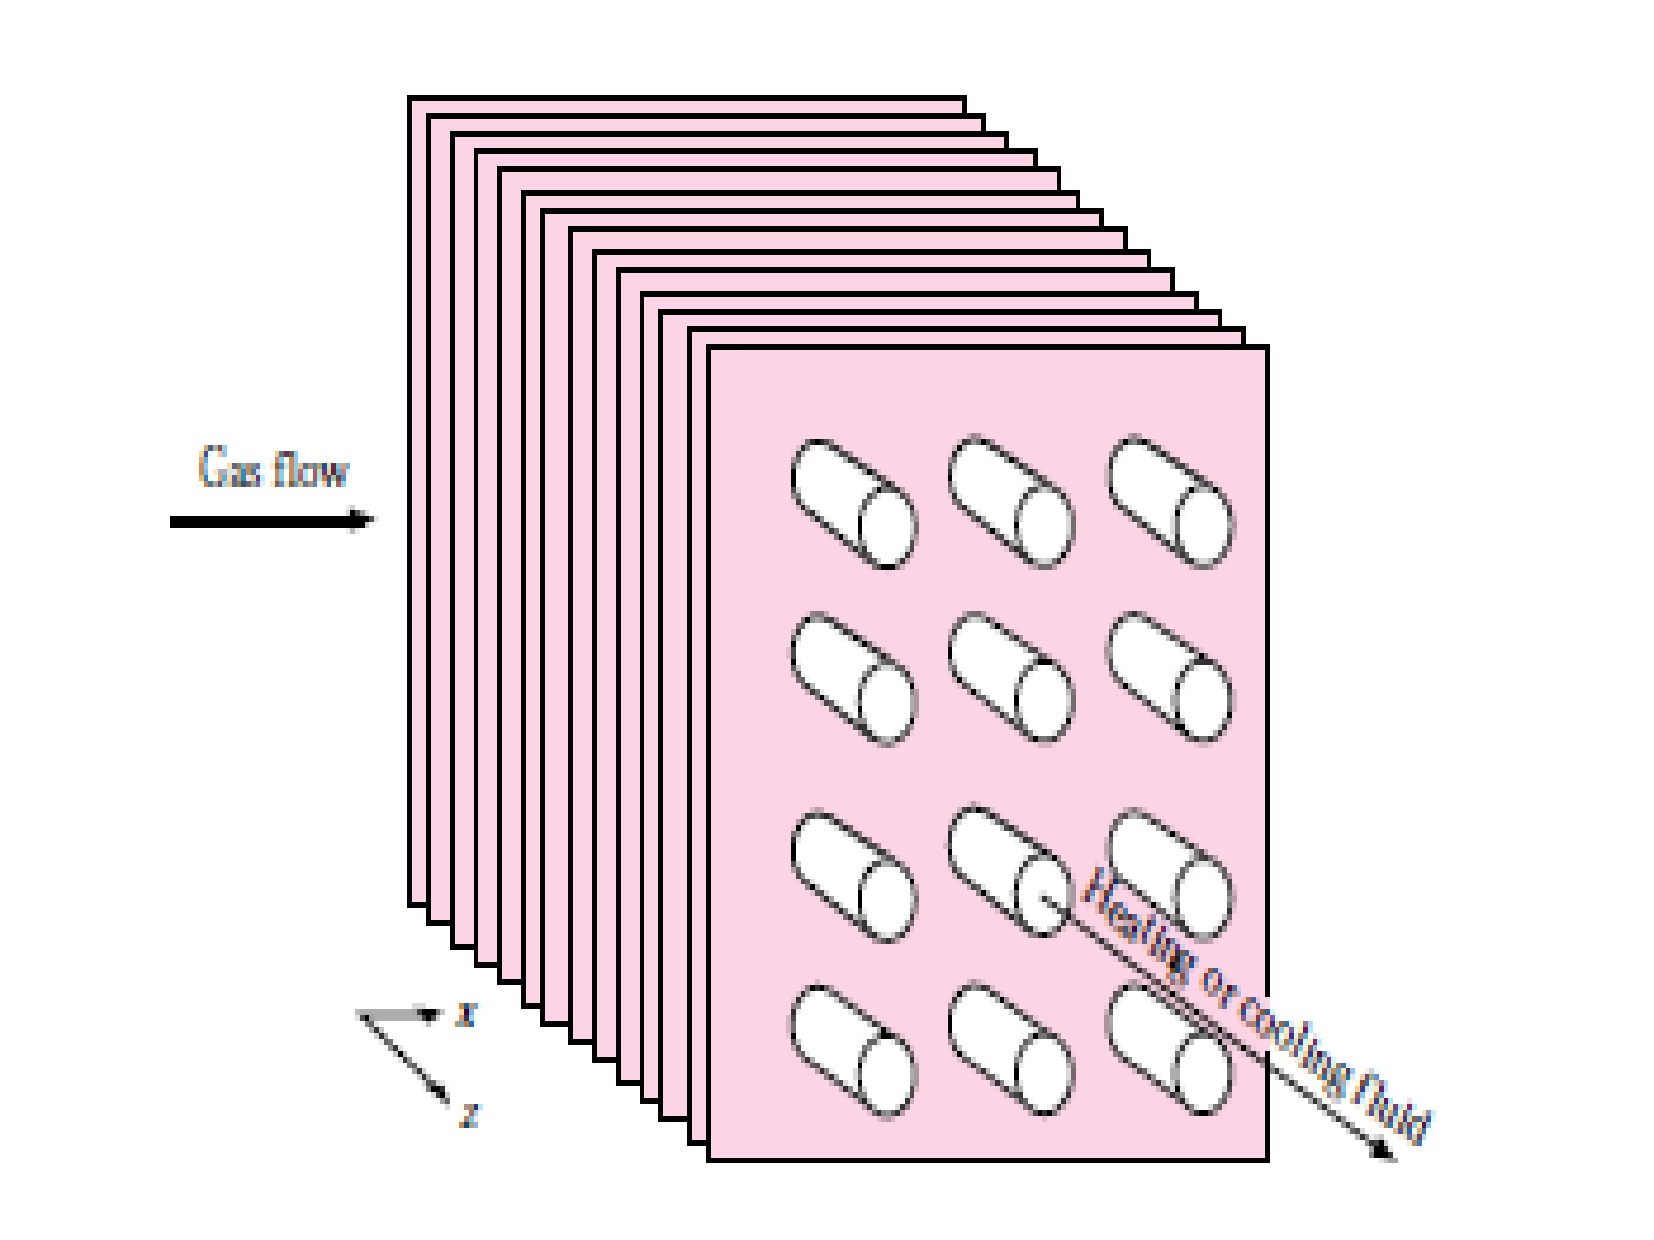
\includegraphics[width=1.1\columnwidth,clip]{./Pics/CrossFlowHE_UnmixedFluids_Example}
       \end{column}
       \begin{column}[l]{0.42\linewidth}
          \begin{enumerate}\setcounter{enumi}{4}
              \item A finned-tube heat exchanger is used to heat 2.36 m$^{3}$/s of air at 1 atm from 15.55 to 29.44$^{\circ}$C. Hot water enters the tubes at 82.22$^{\circ}$C, and the air flows across the tubes, producing an average overall heat-transfer coefficient of 227 W/(m$^{2}$.$^{\circ}$C). The total surface area of the exchanger 9.29 m$^{2}$. Calculate the exit water temperature and the heat-transfer rate.
          \end{enumerate}
       \end{column}      
    \end{columns}
\end{frame}



%%%
%%%  SECTION
%%%
\section{Summary}


%%% Slide 
%%%
\begin{frame}
  \frametitle{Summary}
    \begin{enumerate}
       \item Main elements and types of heat exchangers;
       \item Main heat transfer mechanisms (fluid-solid-fluid) in HE of common design;
       \item Study of overall heat transfer coefficient;
       \item LMTD method for HE design;
       \item $\epsilon$-NTU methods for HE design.
    \end{enumerate}
\end{frame}








%%%
%%% Appendix
%%%
\section{Appendices}

\subsection{Appendix 1: Correction-factor plot for LMTD Method}\label{appendix1}


{
  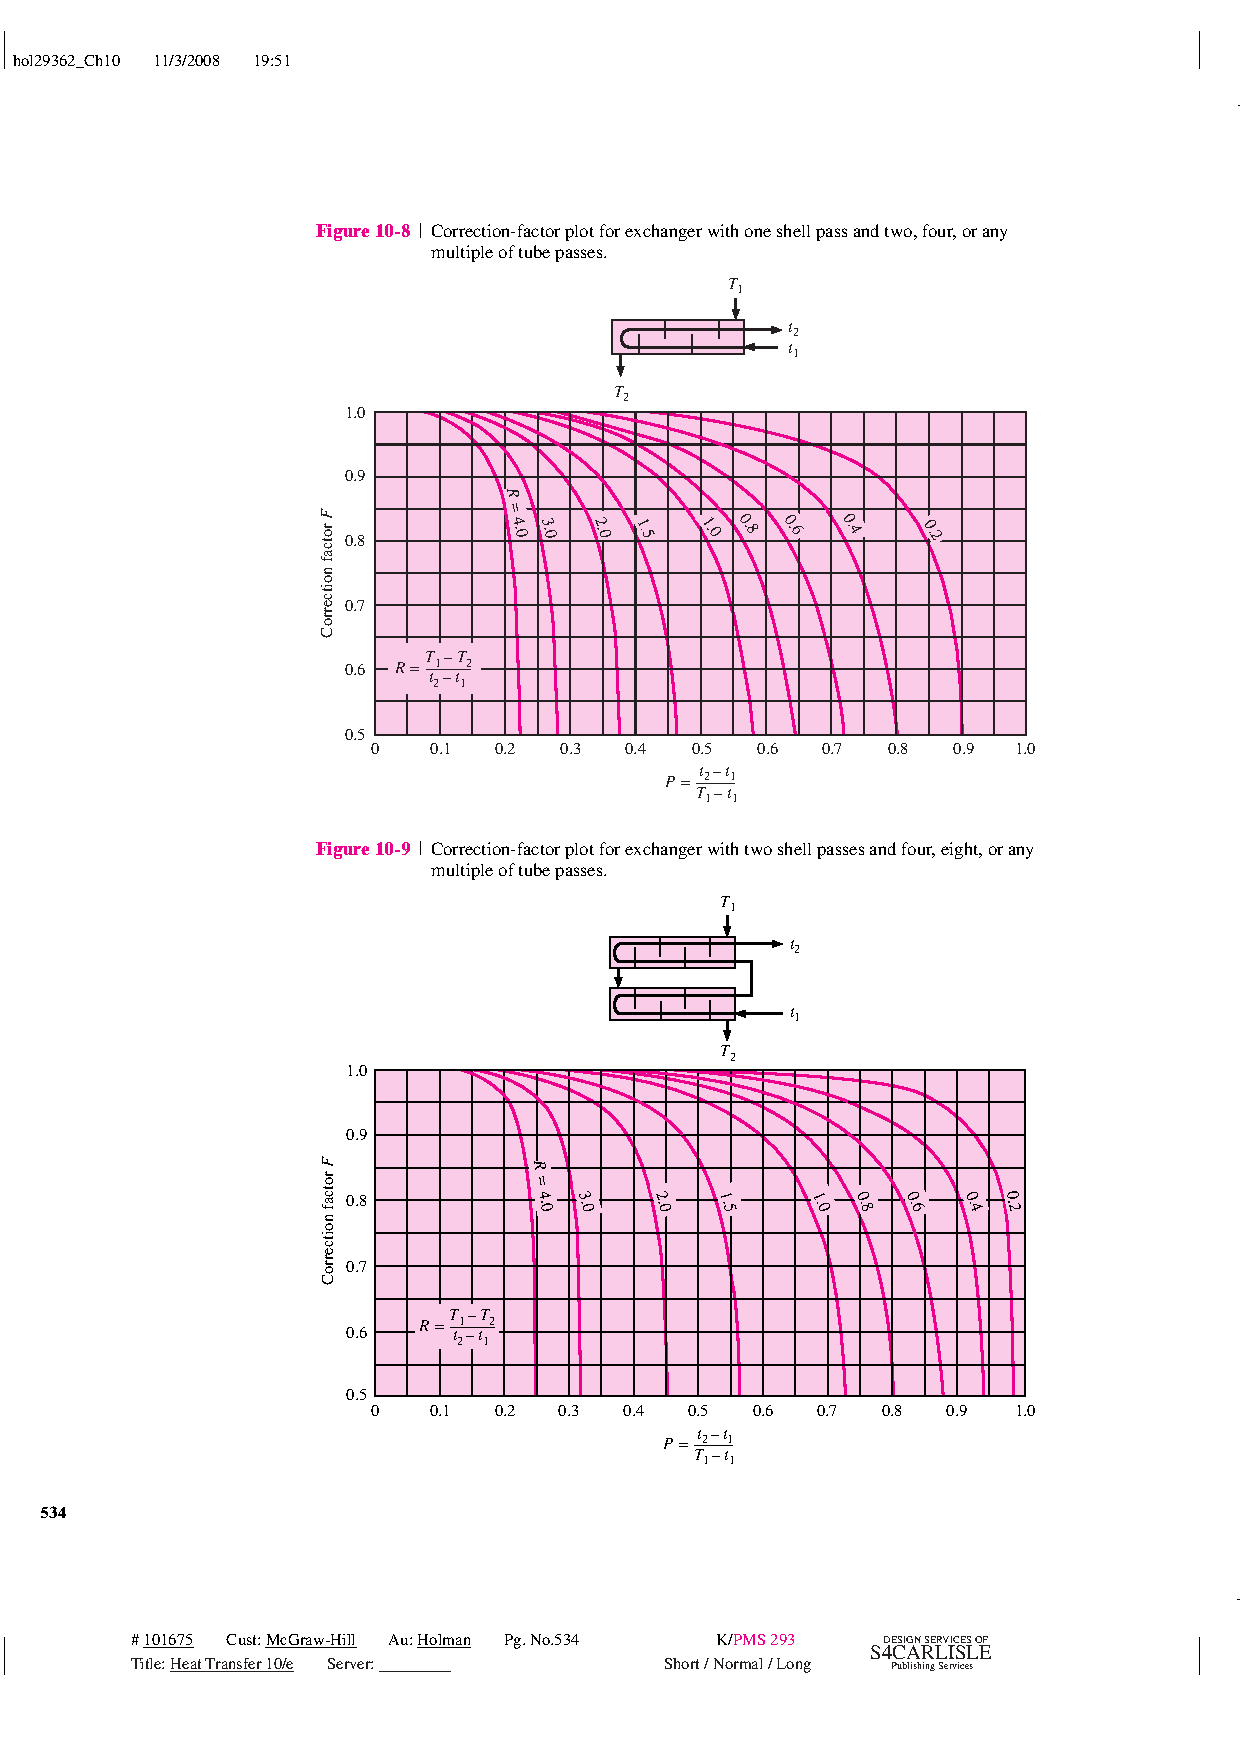
\includepdf[pages=-,fitpaper]{./Pics/LMTD_Plot.pdf}
}
%%%
%%% Slide
%%%
\begin{frame}
 \frametitle{Correction-factor plot for LMTD Method}
        \begin{center}
          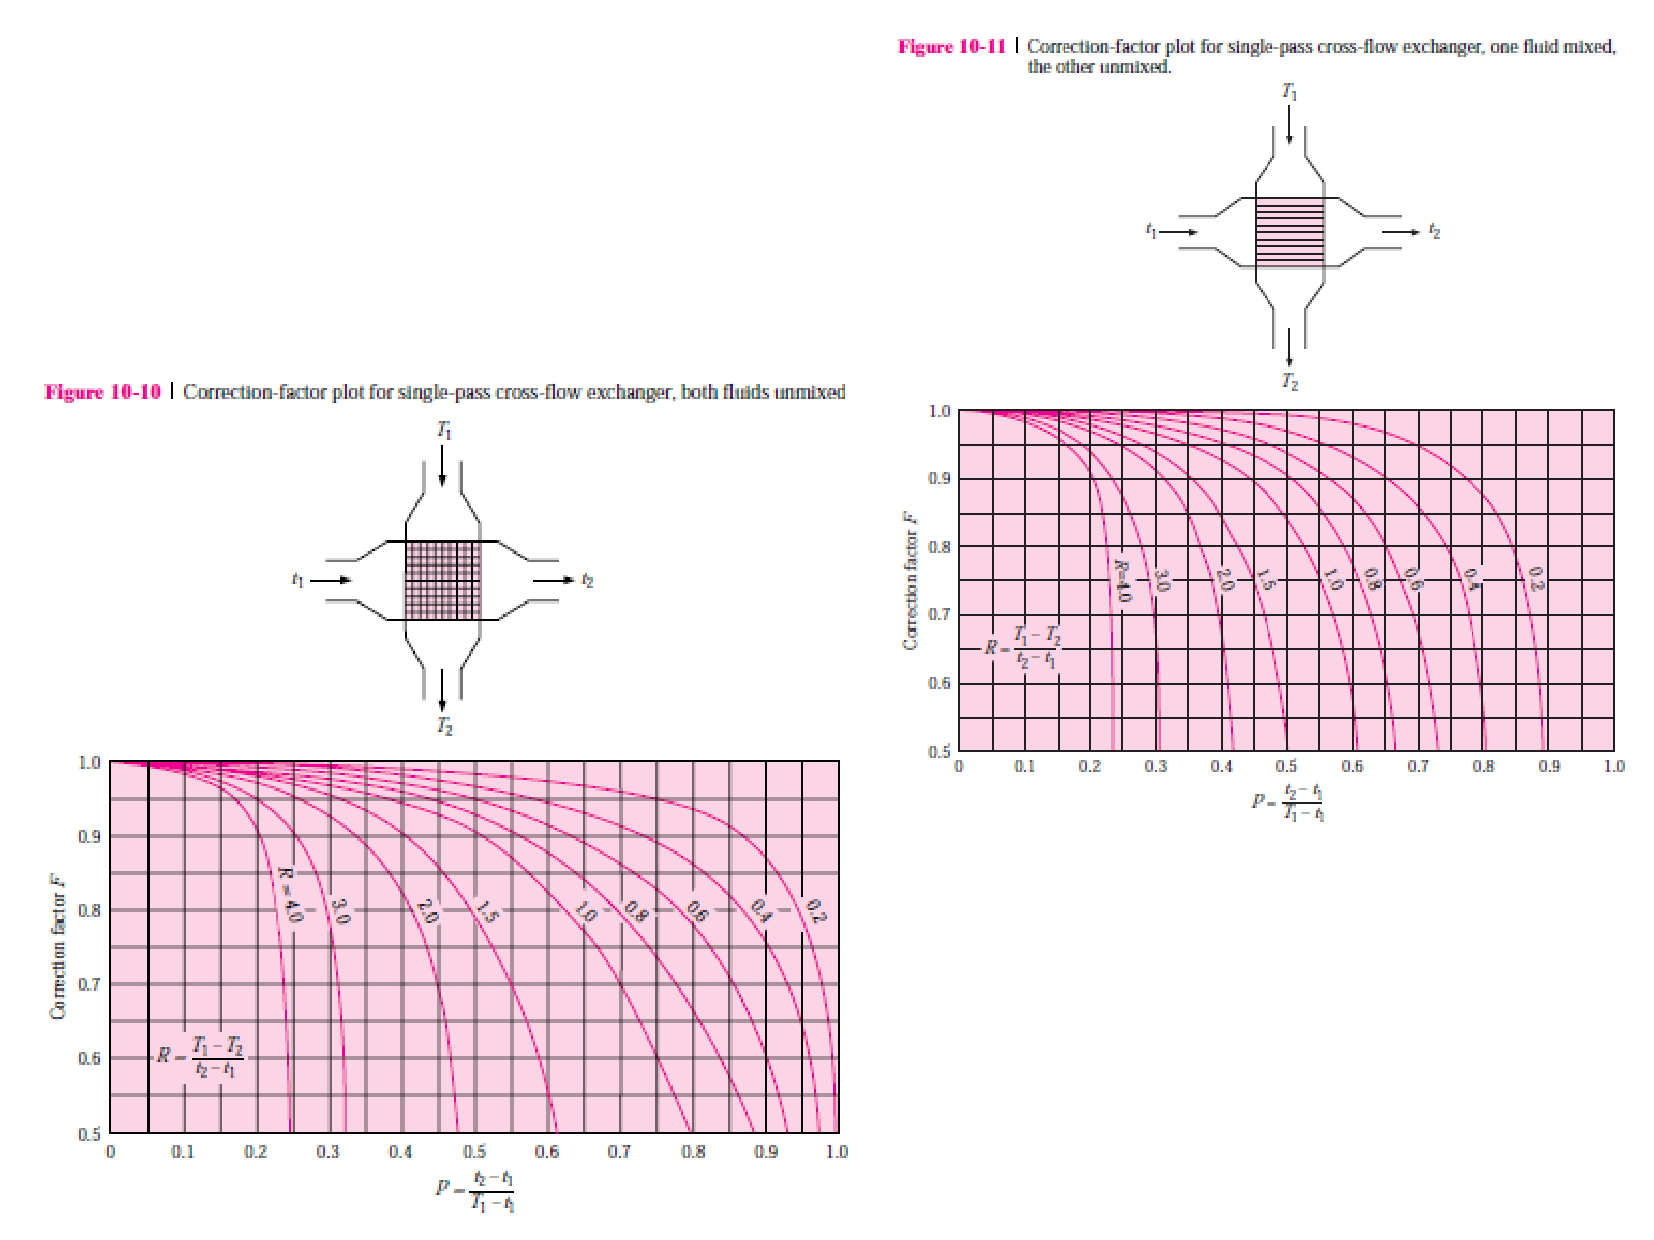
\includegraphics[width=.9\columnwidth,height=.65\columnwidth,clip]{./Pics/LMTD_Plot2}
        \end{center}
\end{frame}
 


%%%
%%% Appendix
%%%
\subsection{Appendix 2: Effectiveness-NTU plots and Expressions}\label{appendix2}


{
  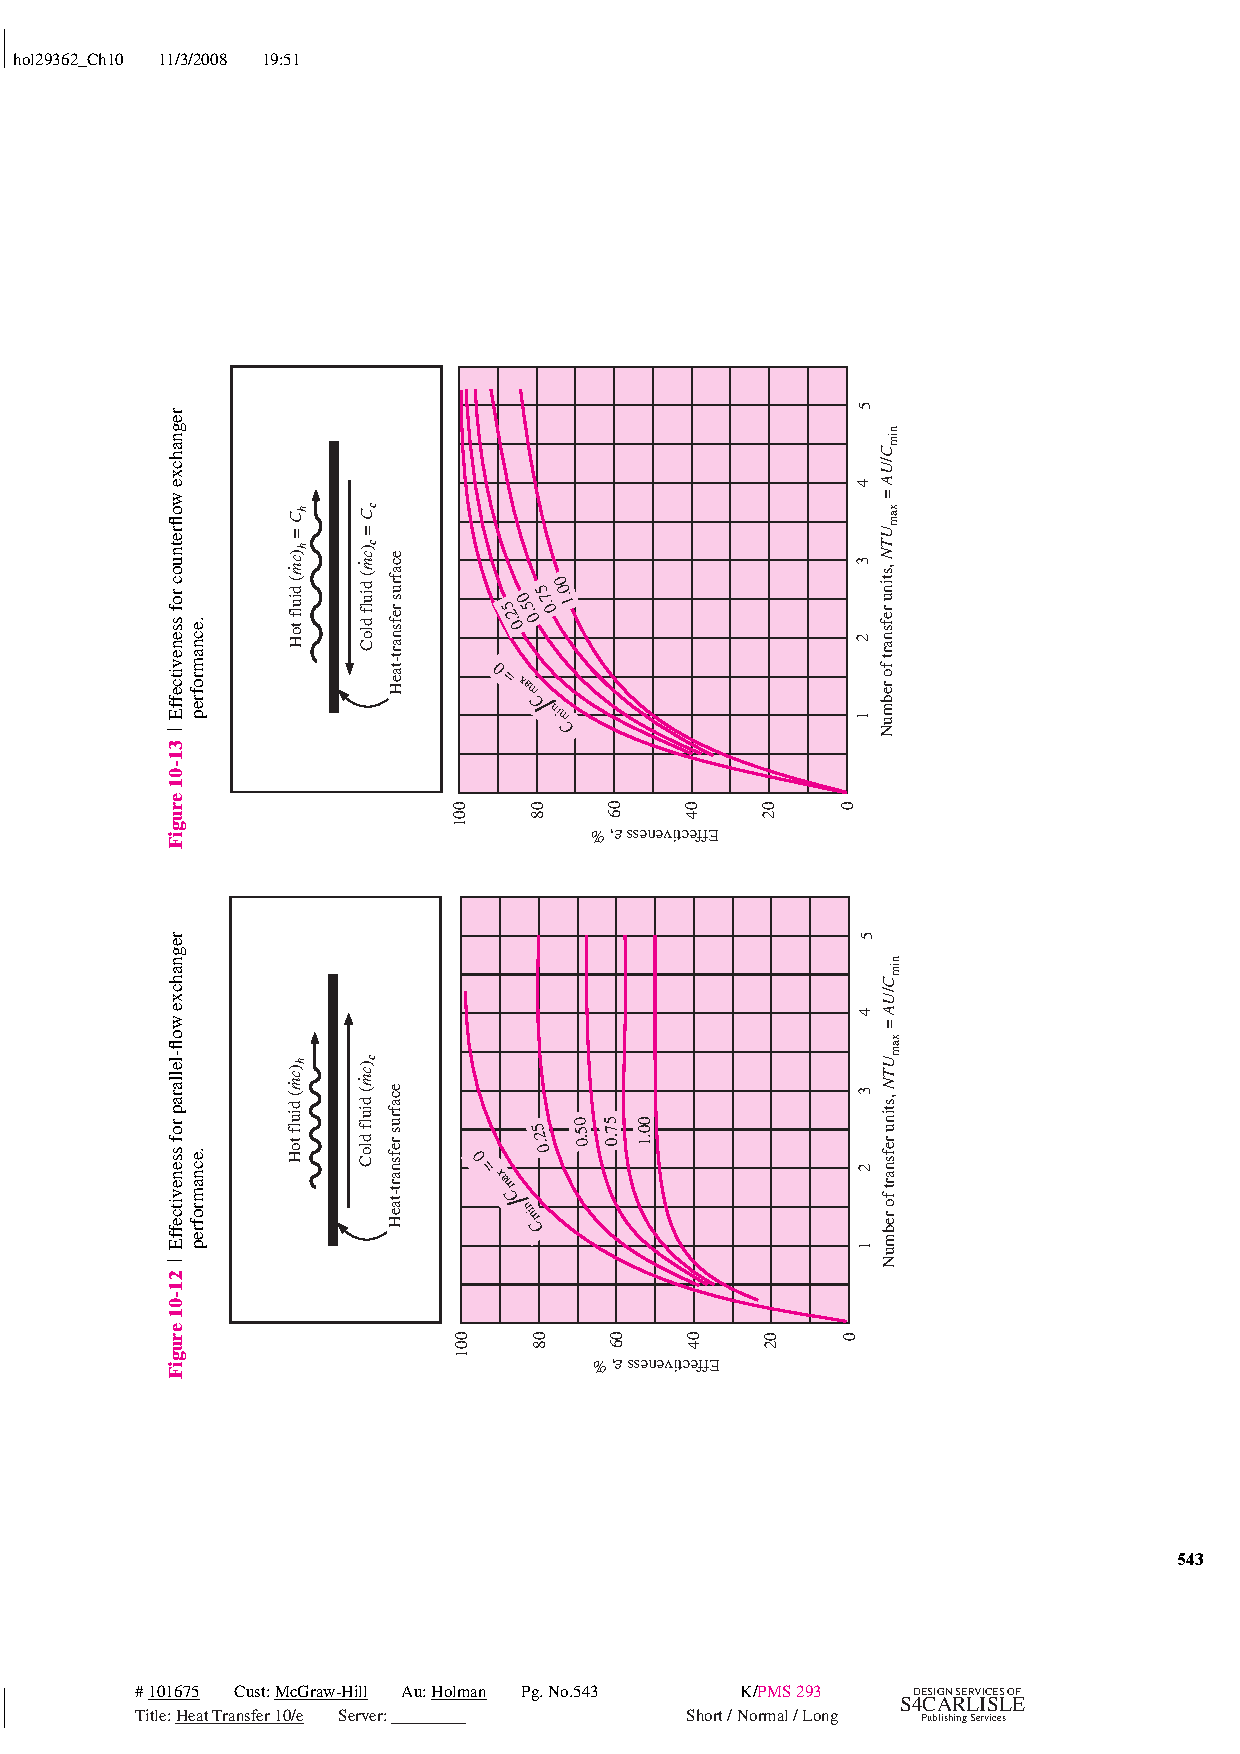
\includepdf[pages=-,fitpaper]{./Pics/NTU.pdf}
}

\end{document}
